\chapter{Project: A Pixel Art Editor}\label{paint}

\epigraphhead[30]{
\epigraph{\hspace*{-.1cm}\itshape``I look at the many colors before me. I look at my blank canvas. Then, I try to apply colors like words that shape poems, like notes that shape music.''}%
{---Joan Miro}
}\index{Miro, Joan}\index{drawing program example}\index{project chapter}

The material from the previous chapters gives you all the elements you need to build a basic \index{web application}web application. In this chapter, we will do just that.\index{file!image}

Our \index{application}application will be a \index{pixel}pixel \index{drawing}drawing program, where you can modify a picture pixel by pixel by manipulating a zoomed-in view of it, shown as a grid of colored squares. You can use the program to open image files, scribble on them with your mouse or other pointer device, and save them. This is what it will look like:

\vskip 1.5ex
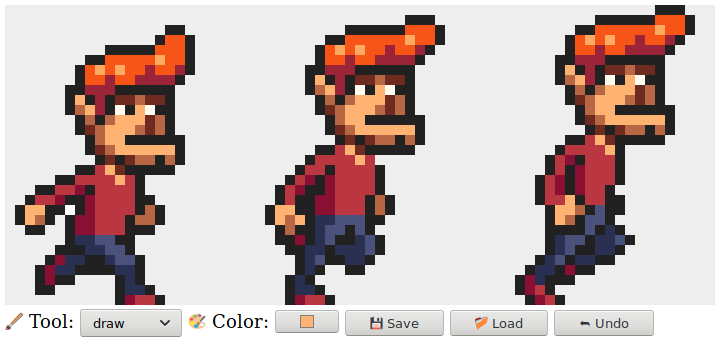
\includegraphics[width=8cm]{img/pixel_editor.png}
\vskip 1.5ex

Painting on a computer is great. You don't need to worry about materials, \index{skill}skill, or talent. You just start smearing.

\section{Components}\index{drawing}\index{select (HTML tag)}\index{canvas (HTML tag)}\index{component}

The interface for the application shows a big \lstinline`<canvas>` element on top, with a number of form \index{field}fields below it. The user draws on the \index{picture}picture by selecting a tool from a \lstinline`<select>` field and then clicking, \index{touch}touching, or \index{dragging}dragging across the canvas. There are \index{tool}tools for drawing single pixels or rectangles, for filling an area, and for picking a \index{color}color from the picture.\index{DOM!components}

We will structure the editor interface as a number of \emph{\index{component}components}, objects that are responsible for a piece of the DOM and that may contain other components inside them.\index{state!of application}

The state of the application consists of the current picture, the selected tool, and the selected color. We'll set things up so that the state lives in a single value, and the interface components always base the way they look on the current state.

To see why this is important, let's consider the alternative—distributing pieces of state throughout the interface. Up to a certain point, this is easier to program. We can just put in a \index{color field}color field and read its value when we need to know the current color.

But then we add the \index{color picker}color picker—a tool that lets you click the picture to select the color of a given pixel. To keep the color field showing the correct color, that tool would have to know that it exists and update it whenever it picks a new color. If you ever add another place that makes the color visible (maybe the mouse cursor could show it), you have to update your color-changing code to keep that synchronized.\index{modularity}

In effect, this creates a problem where each part of the interface needs to know about all other parts, which is not very modular. For small applications like the one in this chapter, that may not be a problem. For bigger projects, it can turn into a real nightmare.

To avoid this nightmare on principle, we're going to be strict about \emph{\index{data flow}data flow}. There is a state, and the interface is drawn based on that state. An interface component may respond to user actions by updating the state, at which point the components get a chance to synchronize themselves with this new state.\index{library}\index{framework}

In practice, each \index{component}component is set up so that when it is given a new state, it also notifies its child components, insofar as those need to be updated. Setting this up is a bit of a hassle. Making this more convenient is the main selling point of many browser programming libraries. But for a small application like this, we can do it without such infrastructure.\index{state!transitions}

Updates to the state are represented as objects, which we'll call \emph{\index{action}actions}. Components may create such actions and \emph{\index{dispatch}dispatch} them—give them to a central state management function. That function computes the next state, after which the interface components update themselves to this new state.\index{DOM!components}

We're taking the messy task of running a \index{user interface}user interface and applying some \index{structure}structure to it. Though the DOM-related pieces are still full of \index{side effect}side effects, they are held up by a conceptually simple backbone: the state update cycle. The state determines what the DOM looks like, and the only way DOM events can change the state is by dispatching actions to the state.\index{data flow}

There are \emph{many} variants of this approach, each with its own benefits and problems, but their central idea is the same: state changes should go through a single well-defined channel, not happen all over the place.\index{dom property}\index{interface!object}

Our \index{component}components will be \index{class}classes conforming to an interface. Their constructor is given a state—which may be the whole application state or some smaller value if it doesn't need access to everything—and uses that to build up a \lstinline`dom` property. This is the DOM element that represents the component. Most constructors will also take some other values that won't change over time, such as the function they can use to \index{dispatch}dispatch an action.\index{syncState method}

Each component has a \lstinline`syncState` method that is used to synchronize it to a new state value. The method takes one argument, the state, which is of the same type as the first argument to its constructor.

\section{The state}\index{Picture class}\index{picture property}\index{tool property}\index{color property}\index{Matrix class}

The application state will be an object with \lstinline`picture`, \lstinline`tool`, and \lstinline`color` properties. The picture is itself an object that stores the width, height, and pixel content of the picture. The \index{pixel}pixels are stored in an array, in the same way as the matrix class from \hyperref[object]{Chapter 6}—row by row, from top to bottom.

\begin{lstlisting}
class Picture {
  constructor(width, height, pixels) {
    this.width = width;
    this.height = height;
    this.pixels = pixels;
  }
  static empty(width, height, color) {
    let pixels = new Array(width * height).fill(color);
    return new Picture(width, height, pixels);
  }
  pixel(x, y) {
    return this.pixels[x + y * this.width];
  }
  draw(pixels) {
    let copy = this.pixels.slice();
    for (let {x, y, color} of pixels) {
      copy[x + y * this.width] = color;
    }
    return new Picture(this.width, this.height, copy);
  }
}
\end{lstlisting}
\noindent\index{side effect}\index{persistent data structure}

We want to be able to treat a picture as an \index{immutable}immutable value, for reasons that we'll get back to later in the chapter. But we also sometimes need to update a whole bunch of pixels at a time. To be able to do that, the class has a \lstinline`draw` method that expects an array of updated pixels—objects with \lstinline`x`, \lstinline`y`, and \lstinline`color` properties—and creates a new picture with those pixels overwritten. This method uses \lstinline`slice` without arguments to copy the entire pixel array—the start of the slice defaults to 0, and the end defaults to the array's length.\index{Array constructor}\index{fill method}\index{length property!for array}\index{array!creation}

The \lstinline`empty` method uses two pieces of array functionality that we haven't seen before. The \lstinline`Array` constructor can be called with a number to create an empty array of the given length. The \lstinline`fill` method can then be used to fill this array with a given value. These are used to create an array in which all pixels have the same color.\index{hexadecimal number}\index{color component}\index{color field}\index{fillColor property}

Colors are stored as strings containing traditional \index{CSS}CSS \index{color
code}color
codes made up of a \index{hash sign}hash sign (\lstinline`#`) followed by six hexadecimal (base-16) digits—two for the \index{red}red component, two for the \index{green}green component, and two for the \index{blue}blue component. This is a somewhat cryptic and inconvenient way to write colors, but it is the format the HTML color input field uses, and it can be used in the \lstinline`fillColor` property of a canvas drawing context, so for the ways we'll use colors in this program, it is practical enough.\index{black}

Black, where all components are zero, is written \lstinline`"#000000"`, and bright \index{pink}pink looks like \lstinline`"#ff00ff"`, where the red and blue components have the maximum value of 255, written \lstinline`ff` in hexadecimal \index{digit}digits (which use \emph{a} to \emph{f} to represent digits 10 to 15).\index{state!transitions}

We'll allow the interface to \index{dispatch}dispatch \index{action}actions as objects whose properties overwrite the properties of the previous state. The color field, when the user changes it, could dispatch an object like \lstinline`{color: field.value}`, from which this update function can compute a new state.\index{updateState function}

\begin{lstlisting}
function updateState(state, action) {
  return Object.assign({}, state, action);
}
\end{lstlisting}
\noindent\index{period character}\index{spread}\index{Object.assign function}

This rather cumbersome pattern, in which \lstinline`Object.assign` is used to first add the properties of \lstinline`state` to an empty object and then overwrite some of those with the properties from \lstinline`action`, is common in JavaScript code that uses \index{immutable}immutable objects. A more convenient notation for this, in which the triple-dot operator is used to include all properties from another object in an object expression, is in the final stages of being standardized. With that addition, you could write \lstinline`{...state, ...action}` instead. At the time of writing, this doesn't yet work in all browsers.

\section{DOM building}\index{createElement method}\index{elt function}\index{DOM!construction}

One of the main things that interface components do is creating DOM structure. We again don't want to directly use the verbose DOM methods for that, so here's a slightly expanded version of the \lstinline`elt` function:

\begin{lstlisting}
function elt(type, props, ...children) {
  let dom = document.createElement(type);
  if (props) Object.assign(dom, props);
  for (let child of children) {
    if (typeof child != "string") dom.appendChild(child);
    else dom.appendChild(document.createTextNode(child));
  }
  return dom;
}
\end{lstlisting}
\noindent\index{setAttribute method}\index{attribute}\index{onclick property}\index{click event}\index{event handling}

The main difference between this version and the one we used in \hyperref[game.domdisplay]{Chapter 16} is that it assigns \emph{properties} to DOM nodes, not \emph{attributes}. This means we can't use it to set arbitrary attributes, but we \emph{can} use it to set properties whose value isn't a string, such as \lstinline`onclick`, which can be set to a function to register a click event handler.\index{button (HTML tag)}

This allows the following style of registering event handlers:

\begin{lstlisting}
<body>
  <script>
    document.body.appendChild(elt("button", {
      onclick: () => console.log("click")
    }, "The button"));
  </script>
</body>
\end{lstlisting}
\noindent

\section{The canvas}

The first component we'll define is the part of the interface that displays the picture as a grid of colored boxes. This component is responsible for two things: showing a picture and communicating \index{pointer event}pointer events on that picture to the rest of the application.\index{PictureCanvas class}\index{callback function}\index{scale constant}\index{canvas (HTML tag)}\index{mousedown event}\index{touchstart event}\index{state!of application}

As such, we can define it as a component that knows about only the current picture, not the whole application state. Because it doesn't know how the application as a whole works, it cannot directly dispatch \index{action}actions. Rather, when responding to pointer events, it calls a callback function provided by the code that created it, which will handle the application-specific parts.

\begin{lstlisting}
const scale = 10;

class PictureCanvas {
  constructor(picture, pointerDown) {
    this.dom = elt("canvas", {
      onmousedown: event => this.mouse(event, pointerDown),
      ontouchstart: event => this.touch(event, pointerDown)
    });
    this.syncState(picture);
  }
  syncState(picture) {
    if (this.picture == picture) return;
    this.picture = picture;
    drawPicture(this.picture, this.dom, scale);
  }
}
\end{lstlisting}
\noindent\index{syncState method}\index{efficiency}

We draw each pixel as a 10-by-10 square, as determined by the \lstinline`scale` constant. To avoid unnecessary work, the component keeps track of its current picture and does a redraw only when \lstinline`syncState` is given a new picture.\index{drawPicture function}

The actual drawing function sets the size of the canvas based on the scale and picture size and fills it with a series of squares, one for each pixel.

\begin{lstlisting}
function drawPicture(picture, canvas, scale) {
  canvas.width = picture.width * scale;
  canvas.height = picture.height * scale;
  let cx = canvas.getContext("2d");

  for (let y = 0; y < picture.height; y++) {
    for (let x = 0; x < picture.width; x++) {
      cx.fillStyle = picture.pixel(x, y);
      cx.fillRect(x * scale, y * scale, scale, scale);
    }
  }
}
\end{lstlisting}
\noindent\index{mousedown event}\index{mousemove event}\index{button property}\index{buttons property}\index{pointerPosition function}

When the left mouse button is pressed while the mouse is over the picture canvas, the component calls the \lstinline`pointerDown` callback, giving it the position of the pixel that was clicked—in picture coordinates. This will be used to implement mouse interaction with the picture. The callback may return another callback function to be notified when the pointer is moved to a different pixel while the button is held down.

\begin{lstlisting}
PictureCanvas.prototype.mouse = function(downEvent, onDown) {
  if (downEvent.button != 0) return;
  let pos = pointerPosition(downEvent, this.dom);
  let onMove = onDown(pos);
  if (!onMove) return;
  let move = moveEvent => {
    if (moveEvent.buttons == 0) {
      this.dom.removeEventListener("mousemove", move);
    } else {
      let newPos = pointerPosition(moveEvent, this.dom);
      if (newPos.x == pos.x && newPos.y == pos.y) return;
      pos = newPos;
      onMove(newPos);
    }
  };
  this.dom.addEventListener("mousemove", move);
};

function pointerPosition(pos, domNode) {
  let rect = domNode.getBoundingClientRect();
  return {x: Math.floor((pos.clientX - rect.left) / scale),
          y: Math.floor((pos.clientY - rect.top) / scale)};
}
\end{lstlisting}
\noindent\index{getBoundingClientRect method}\index{clientX property}\index{clientY property}

Since we know the size of the \index{pixel}pixels and we can use \lstinline`getBoundingClientRect` to find the position of the canvas on the screen, it is possible to go from mouse event coordinates (\lstinline`clientX` and \lstinline`clientY`) to picture coordinates. These are always rounded down so that they refer to a specific pixel.\index{touchstart event}\index{touchmove event}\index{preventDefault method}

With touch events, we have to do something similar, but using different events and making sure we call \lstinline`preventDefault` on the \lstinline`"touchstart"` event to prevent \index{panning}panning.

\begin{lstlisting}
PictureCanvas.prototype.touch = function(startEvent,
                                         onDown) {
  let pos = pointerPosition(startEvent.touches[0], this.dom);
  let onMove = onDown(pos);
  startEvent.preventDefault();
  if (!onMove) return;
  let move = moveEvent => {
    let newPos = pointerPosition(moveEvent.touches[0],
                                 this.dom);
    if (newPos.x == pos.x && newPos.y == pos.y) return;
    pos = newPos;
    onMove(newPos);
  };
  let end = () => {
    this.dom.removeEventListener("touchmove", move);
    this.dom.removeEventListener("touchend", end);
  };
  this.dom.addEventListener("touchmove", move);
  this.dom.addEventListener("touchend", end);
};
\end{lstlisting}
\noindent\index{touches property}\index{clientX property}\index{clientY property}

For touch events, \lstinline`clientX` and \lstinline`clientY` aren't available directly on the event object, but we can use the coordinates of the first touch object in the \lstinline`touches` property.

\section{The application}

To make it possible to build the application piece by piece, we'll implement the main component as a shell around a picture canvas and a dynamic set of \index{tool}tools and \index{control}controls that we pass to its constructor.

The \emph{controls} are the interface elements that appear below the picture. They'll be provided as an array of \index{component}component constructors.\index{br (HTML tag)}\index{flood fill}\index{select (HTML tag)}\index{PixelEditor class}\index{dispatch}

The \emph{tools} do things like drawing pixels or filling in an area. The application shows the set of available tools as a \lstinline`<select>` field. The currently selected tool determines what happens when the user interacts with the picture with a pointer device. The set of available tools is provided as an object that maps the names that appear in the drop-down field to functions that implement the tools. Such functions get a picture position, a current application state, and a \lstinline`dispatch` function as arguments. They may return a move handler function that gets called with a new position and a current state when the pointer moves to a different pixel.

\begin{lstlisting}
class PixelEditor {
  constructor(state, config) {
    let {tools, controls, dispatch} = config;
    this.state = state;

    this.canvas = new PictureCanvas(state.picture, pos => {
      let tool = tools[this.state.tool];
      let onMove = tool(pos, this.state, dispatch);
      if (onMove) return pos => onMove(pos, this.state);
    });
    this.controls = controls.map(
      Control => new Control(state, config));
    this.dom = elt("div", {}, this.canvas.dom, elt("br"),
                   ...this.controls.reduce(
                     (a, c) => a.concat(" ", c.dom), []));
  }
  syncState(state) {
    this.state = state;
    this.canvas.syncState(state.picture);
    for (let ctrl of this.controls) ctrl.syncState(state);
  }
}
\end{lstlisting}
\noindent

The pointer handler given to \lstinline`PictureCanvas` calls the currently selected tool with the appropriate arguments and, if that returns a move handler, adapts it to also receive the state.\index{reduce method}\index{map method}\index{whitespace!in HTML}\index{syncState method}

All controls are constructed and stored in \lstinline`this.controls` so that they can be updated when the application state changes. The call to \lstinline`reduce` introduces spaces between the controls' DOM elements. That way they don't look so pressed together.\index{select (HTML tag)}\index{change event}\index{ToolSelect class}\index{syncState method}

The first control is the \index{tool}tool selection menu. It creates a \lstinline`<select>` element with an option for each tool and sets up a \lstinline`"change"` event handler that updates the application state when the user selects a different tool.

\begin{lstlisting}
class ToolSelect {
  constructor(state, {tools, dispatch}) {
    this.select = elt("select", {
      onchange: () => dispatch({tool: this.select.value})
    }, ...Object.keys(tools).map(name => elt("option", {
      selected: name == state.tool
    }, name)));
    this.dom = elt("label", null, "$<🖌>$ Tool: ", this.select);
  }
  syncState(state) { this.select.value = state.tool; }
}
\end{lstlisting}
\noindent\index{label (HTML tag)}

By wrapping the label text and the field in a \lstinline`<label>` element, we tell the browser that the label belongs to that field so that you can, for example, click the label to focus the field.\index{color field}\index{input (HTML tag)}

We also need to be able to change the color, so let's add a control for that. An HTML \lstinline`<input>` element with a \lstinline`type` attribute of \lstinline`color` gives us a form field that is specialized for selecting colors. Such a field's value is always a CSS color code in \lstinline`"#RRGGBB"` format (red, green, and blue components, two digits per color). The browser will show a \index{color picker}color picker interface when the user interacts with it.

Depending on the browser, the color picker might look like this:

\vskip 1.5ex
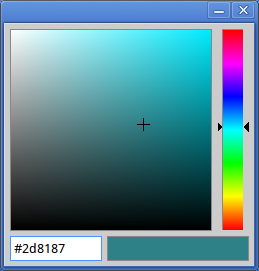
\includegraphics[width=6cm]{img/color-field.png}
\vskip 1.5ex\index{ColorSelect class}\index{syncState method}

This \index{control}control creates such a field and wires it up to stay synchronized with the application state's \lstinline`color` property.

\begin{lstlisting}
class ColorSelect {
  constructor(state, {dispatch}) {
    this.input = elt("input", {
      type: "color",
      value: state.color,
      onchange: () => dispatch({color: this.input.value})
    });
    this.dom = elt("label", null, "$<🎨>$ Color: ", this.input);
  }
  syncState(state) { this.input.value = state.color; }
}
\end{lstlisting}
\noindent

\section{Drawing tools}

Before we can draw anything, we need to implement the \index{tool}tools that will control the functionality of mouse or touch events on the canvas.\index{draw function}

The most basic tool is the draw tool, which changes any \index{pixel}pixel you click or tap to the currently selected color. It dispatches an action that updates the picture to a version in which the pointed-at pixel is given the currently selected color.

\begin{lstlisting}
function draw(pos, state, dispatch) {
  function drawPixel({x, y}, state) {
    let drawn = {x, y, color: state.color};
    dispatch({picture: state.picture.draw([drawn])});
  }
  drawPixel(pos, state);
  return drawPixel;
}
\end{lstlisting}
\noindent

The function immediately calls the \lstinline`drawPixel` function but then also returns it so that it is called again for newly touched pixels when the user drags or \index{swipe}swipes over the picture.\index{rectangle function}

To draw larger shapes, it can be useful to quickly create \index{rectangle}rectangles. The \lstinline`rectangle` \index{tool}tool draws a rectangle between the point where you start \index{dragging}dragging and the point that you drag to.

\begin{lstlisting}
function rectangle(start, state, dispatch) {
  function drawRectangle(pos) {
    let xStart = Math.min(start.x, pos.x);
    let yStart = Math.min(start.y, pos.y);
    let xEnd = Math.max(start.x, pos.x);
    let yEnd = Math.max(start.y, pos.y);
    let drawn = [];
    for (let y = yStart; y <= yEnd; y++) {
      for (let x = xStart; x <= xEnd; x++) {
        drawn.push({x, y, color: state.color});
      }
    }
    dispatch({picture: state.picture.draw(drawn)});
  }
  drawRectangle(start);
  return drawRectangle;
}
\end{lstlisting}
\noindent\index{persistent data structure}\index{state!persistence}

An important detail in this implementation is that when dragging, the rectangle is redrawn on the picture from the \emph{original} state. That way, you can make the rectangle larger and smaller again while creating it, without the intermediate rectangles sticking around in the final picture. This is one of the reasons why \index{immutable}immutable picture objects are useful—we'll see another reason later.

Implementing \index{flood fill}flood fill is somewhat more involved. This is a \index{tool}tool that fills the pixel under the pointer and all adjacent pixels that have the same color. ``Adjacent'' means directly horizontally or vertically adjacent, not diagonally. This picture illustrates the set of \index{pixel}pixels colored when the flood fill tool is used at the marked pixel:

\vskip 1.5ex
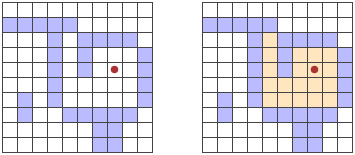
\includegraphics[width=6cm]{img/generated/flood-grid.pdf}
\vskip 1.5ex\index{fill function}

Interestingly, the way we'll do this looks a bit like the \index{pathfinding}pathfinding code from \hyperref[robot]{Chapter 7}. Whereas that code searched through a graph to find a route, this code searches through a grid to find all ``connected'' pixels. The problem of keeping track of a branching set of possible routes is similar.

\begin{lstlisting}
const around = [{dx: -1, dy: 0}, {dx: 1, dy: 0},
                {dx: 0, dy: -1}, {dx: 0, dy: 1}];

function fill({x, y}, state, dispatch) {
  let targetColor = state.picture.pixel(x, y);
  let drawn = [{x, y, color: state.color}];
  for (let done = 0; done < drawn.length; done++) {
    for (let {dx, dy} of around) {
      let x = drawn[done].x + dx, y = drawn[done].y + dy;
      if (x >= 0 && x < state.picture.width &&
          y >= 0 && y < state.picture.height &&
          state.picture.pixel(x, y) == targetColor &&
          !drawn.some(p => p.x == x && p.y == y)) {
        drawn.push({x, y, color: state.color});
      }
    }
  }
  dispatch({picture: state.picture.draw(drawn)});
}
\end{lstlisting}
\noindent

The array of drawn pixels doubles as the function's \index{work list}work list. For each pixel reached, we have to see whether any adjacent pixels have the same color and haven't already been painted over. The loop counter lags behind the length of the \lstinline`drawn` array as new pixels are added. Any pixels ahead of it still need to be explored. When it catches up with the length, no unexplored pixels remain, and the function is done.\index{pick function}

The final \index{tool}tool is a \index{color picker}color picker, which allows you to point at a color in the picture to use it as the current drawing color.

\begin{lstlisting}
function pick(pos, state, dispatch) {
  dispatch({color: state.picture.pixel(pos.x, pos.y)});
}
\end{lstlisting}
\noindent

\section{Saving and loading}\index{SaveButton class}\index{drawPicture function}\index{file!image}

When we've drawn our masterpiece, we'll want to save it for later. We should add a button for \index{download}downloading the current picture as an image file. This \index{control}control provides that button:

\begin{lstlisting}
class SaveButton {
  constructor(state) {
    this.picture = state.picture;
    this.dom = elt("button", {
      onclick: () => this.save()
    }, "$<💾>$ Save");
  }
  save() {
    let canvas = elt("canvas");
    drawPicture(this.picture, canvas, 1);
    let link = elt("a", {
      href: canvas.toDataURL(),
      download: "pixelart.png"
    });
    document.body.appendChild(link);
    link.click();
    link.remove();
  }
  syncState(state) { this.picture = state.picture; }
}
\end{lstlisting}
\noindent\index{canvas (HTML tag)}

The component keeps track of the current picture so that it can access it when saving. To create the image file, it uses a \lstinline`<canvas>` element that it draws the picture on (at a scale of one pixel per pixel).\index{toDataURL method}\index{data URL}

The \lstinline`toDataURL` method on a canvas element creates a URL that starts with \lstinline`data:`. Unlike \lstinline`http:` and \lstinline`https:` URLs, data URLs contain the whole resource in the URL. They are usually very long, but they allow us to create working links to arbitrary pictures, right here in the browser.\index{a (HTML tag)}\index{download attribute}

To actually get the browser to download the picture, we then create a \index{link}link element that points at this URL and has a \lstinline`download` attribute. Such links, when clicked, make the browser show a file save dialog. We add that link to the document, simulate a click on it, and remove it again.

You can do a lot with \index{browser}browser technology, but sometimes the way to do it is rather odd.\index{LoadButton class}\index{control}\index{file!image}

And it gets worse. We'll also want to be able to load existing image files into our application. To do that, we again define a button component.

\begin{lstlisting}
class LoadButton {
  constructor(_, {dispatch}) {
    this.dom = elt("button", {
      onclick: () => startLoad(dispatch)
    }, "$<📁>$ Load");
  }
  syncState() {}
}

function startLoad(dispatch) {
  let input = elt("input", {
    type: "file",
    onchange: () => finishLoad(input.files[0], dispatch)
  });
  document.body.appendChild(input);
  input.click();
  input.remove();
}
\end{lstlisting}
\noindent\index{file!access}\index{input (HTML tag)}

To get access to a file on the user's computer, we need the user to select the file through a file input field. But I don't want the load button to look like a file input field, so we create the file input when the button is clicked and then pretend that this file input itself was clicked.\index{FileReader class}\index{img (HTML tag)}\index{readAsDataURL method}\index{Picture class}

When the user has selected a file, we can use \lstinline`FileReader` to get access to its contents, again as a \index{data URL}data URL. That URL can be used to create an \lstinline`<img>` element, but because we can't get direct access to the pixels in such an image, we can't create a \lstinline`Picture` object from that.

\begin{lstlisting}
function finishLoad(file, dispatch) {
  if (file == null) return;
  let reader = new FileReader();
  reader.addEventListener("load", () => {
    let image = elt("img", {
      onload: () => dispatch({
        picture: pictureFromImage(image)
      }),
      src: reader.result
    });
  });
  reader.readAsDataURL(file);
}
\end{lstlisting}
\noindent\index{canvas (HTML tag)}\index{getImageData method}\index{pictureFromImage function}

To get access to the pixels, we must first draw the picture to a \lstinline`<canvas>` element. The canvas context has a \lstinline`getImageData` method that allows a script to read its \index{pixel}pixels. So, once the picture is on the canvas, we can access it and construct a \lstinline`Picture` object.

\begin{lstlisting}
function pictureFromImage(image) {
  let width = Math.min(100, image.width);
  let height = Math.min(100, image.height);
  let canvas = elt("canvas", {width, height});
  let cx = canvas.getContext("2d");
  cx.drawImage(image, 0, 0);
  let pixels = [];
  let {data} = cx.getImageData(0, 0, width, height);

  function hex(n) {
    return n.toString(16).padStart(2, "0");
  }
  for (let i = 0; i < data.length; i += 4) {
    let [r, g, b] = data.slice(i, i + 3);
    pixels.push("#" + hex(r) + hex(g) + hex(b));
  }
  return new Picture(width, height, pixels);
}
\end{lstlisting}
\noindent

We'll limit the size of images to 100 by 100 pixels since anything bigger will look \emph{huge} on our display and might slow down the interface.\index{getImageData method}\index{color}\index{transparency}

The \lstinline`data` property of the object returned by \lstinline`getImageData` is an array of color components. For each pixel in the rectangle specified by the arguments, it contains four values, which represent the red, green, blue, and \emph{\index{alpha}alpha} components of the pixel's color, as numbers between 0 and 255. The alpha part represents opacity—when it is zero, the pixel is fully transparent, and when it is 255, it is fully opaque. For our purpose, we can ignore it.\index{hexadecimal number}\index{toString method}

The two hexadecimal digits per component, as used in our color notation, correspond precisely to the 0 to 255 range—two base-16 digits can express 16\textsuperscript{2} = 256 different numbers. The \lstinline`toString` method of numbers can be given a base as argument, so \lstinline`n.toString(16)` will produce a string representation in base 16. We have to make sure that each number takes up two digits, so the \lstinline`hex` helper function calls \lstinline`padStart` to add a leading zero when necessary.

We can load and save now! That leaves one more feature before we're done.

\section{Undo history}

Half of the process of editing is making little mistakes and correcting them. So an important feature in a drawing program is an \index{undo history}undo history.\index{persistent data structure}\index{state!of application}

To be able to undo changes, we need to store previous versions of the picture. Since it's an \index{immutable}immutable value, that is easy. But it does require an additional field in the application state.\index{done property}

We'll add a \lstinline`done` array to keep previous versions of the \index{picture}picture. Maintaining this property requires a more complicated state update function that adds pictures to the array.\index{doneAt property}\index{historyUpdateState function}\index{Date.now function}

But we don't want to store \emph{every} change, only changes a certain amount of \index{time}time apart. To be able to do that, we'll need a second property, \lstinline`doneAt`, tracking the time at which we last stored a picture in the history.

\begin{lstlisting}
function historyUpdateState(state, action) {
  if (action.undo == true) {
    if (state.done.length == 0) return state;
    return Object.assign({}, state, {
      picture: state.done[0],
      done: state.done.slice(1),
      doneAt: 0
    });
  } else if (action.picture &&
             state.doneAt < Date.now() - 1000) {
    return Object.assign({}, state, action, {
      done: [state.picture, ...state.done],
      doneAt: Date.now()
    });
  } else {
    return Object.assign({}, state, action);
  }
}
\end{lstlisting}
\noindent\index{undo history}

When the action is an undo action, the function takes the most recent picture from the history and makes that the current picture. It sets \lstinline`doneAt` to zero so that the next change is guaranteed to store the picture back in the history, allowing you to revert to it another time if you want.

Otherwise, if the action contains a new picture and the last time we stored something is more than a second (1000 milliseconds) ago, the \lstinline`done` and \lstinline`doneAt` properties are updated to store the previous picture.\index{UndoButton class}\index{control}

The undo button \index{component}component doesn't do much. It dispatches undo actions when clicked and disables itself when there is nothing to undo.

\begin{lstlisting}
class UndoButton {
  constructor(state, {dispatch}) {
    this.dom = elt("button", {
      onclick: () => dispatch({undo: true}),
      disabled: state.done.length == 0
    }, "$<⮪>$ Undo");
  }
  syncState(state) {
    this.dom.disabled = state.done.length == 0;
  }
}
\end{lstlisting}
\noindent

\section{Let's draw}\index{PixelEditor class}\index{startState constant}\index{baseTools constant}\index{baseControls constant}\index{startPixelEditor function}

To set up the application, we need to create a state, a set of \index{tool}tools, a set of \index{control}controls, and a \index{dispatch}dispatch function. We can pass them to the \lstinline`PixelEditor` constructor to create the main component. Since we'll need to create several editors in the exercises, we first define some bindings.

\begin{lstlisting}
const startState = {
  tool: "draw",
  color: "#000000",
  picture: Picture.empty(60, 30, "#f0f0f0"),
  done: [],
  doneAt: 0
};

const baseTools = {draw, fill, rectangle, pick};

const baseControls = [
  ToolSelect, ColorSelect, SaveButton, LoadButton, UndoButton
];

function startPixelEditor({state = startState,
                           tools = baseTools,
                           controls = baseControls}) {
  let app = new PixelEditor(state, {
    tools,
    controls,
    dispatch(action) {
      state = historyUpdateState(state, action);
      app.syncState(state);
    }
  });
  return app.dom;
}
\end{lstlisting}
\noindent\index{destructuring binding}\index{= operator}\index{property!access}

When destructuring an object or array, you can use \lstinline`=` after a binding name to give the binding a \index{default value}default value, which is used when the property is missing or holds \lstinline`undefined`. The \lstinline`startPixelEditor` function makes use of this to accept an object with a number of optional properties as an argument. If you don't provide a \lstinline`tools` property, for example, \lstinline`tools` will be bound to \lstinline`baseTools`.

This is how we get an actual editor on the screen:

\begin{lstlisting}
<div></div>
<script>
  document.querySelector("div")
    .appendChild(startPixelEditor({}));
</script>
\end{lstlisting}
\noindent

\section{Why is this so hard?}

Browser technology is amazing. It provides a powerful set of interface building blocks, ways to style and manipulate them, and tools to inspect and debug your applications. The software you write for the \index{browser}browser can be run on almost every computer and phone on the planet.

At the same time, browser technology is ridiculous. You have to learn a large number of silly tricks and obscure facts to master it, and the default programming model it provides is so problematic that most programmers prefer to cover it in several layers of \index{abstraction}abstraction rather than deal with it directly.\index{standard}\index{evolution}

And though the situation is definitely improving, it mostly does so in the form of more elements being added to address shortcomings—creating even more \index{complexity}complexity. A feature used by a million websites can't really be replaced. Even if it could, it would be hard to decide what it should be replaced with.\index{social factors}\index{economic factors}\index{history}

Technology never exists in a vacuum—we're constrained by our tools and the social, economic, and historical factors that produced them. This can be annoying, but it is generally more productive to try to build a good understanding of how the \emph{existing} technical reality works—and why it is the way it is—than to rage against it or hold out for another reality.

New \index{abstraction}abstractions \emph{can} be helpful. The component model and \index{data
flow}data
flow convention I used in this chapter is a crude form of that. As mentioned, there are libraries that try to make user interface programming more pleasant. At the time of writing, \href{https://reactjs.org/}{React} and \href{https://angular.io/}{Angular} are popular choices, but there's a whole cottage industry of such frameworks. If you're interested in programming web applications, I recommend investigating a few of them to understand how they work and what benefits they provide.

\section{Exercises}

There is still room for improvement in our program. Let's add a few more features as exercises.

\subsection{Keyboard bindings}\index{keyboard bindings (exercise)}

Add \index{keyboard}keyboard shortcuts to the application. The first letter of a tool's name selects the tool, and \textsc{control}-Z or \textsc{command}-Z activates undo.\index{PixelEditor class}\index{tabindex attribute}\index{elt function}\index{keydown event}

Do this by modifying the \lstinline`PixelEditor` component. Add a \lstinline`tabIndex` property of 0 to the wrapping \lstinline`<div>` element so that it can receive keyboard \index{focus}focus. Note that the \emph{property} corresponding to the \lstinline`tabindex` \emph{attribute} is called \lstinline`tabIndex`, with a capital I, and our \lstinline`elt` function expects property names. Register the key event handlers directly on that element. This means you have to click, touch, or tab to the application before you can interact with it with the keyboard.\index{ctrlKey property}\index{metaKey property}\index{control key}\index{command key}

Remember that keyboard events have \lstinline`ctrlKey` and \lstinline`metaKey` (for the \textsc{command} key on Mac) properties that you can use to see whether those keys are held down.

\subsection{Efficient drawing}\index{efficient drawing (exercise)}\index{canvas (HTML tag)}\index{efficiency}

During drawing, the majority of work that our application does happens in \lstinline`drawPicture`. Creating a new state and updating the rest of the DOM isn't very expensive, but repainting all the pixels on the canvas is quite a bit of work.\index{syncState method}\index{PictureCanvas class}

Find a way to make the \lstinline`syncState` method of \lstinline`PictureCanvas` faster by redrawing only the pixels that actually changed.\index{drawPicture function}\index{compatibility}

Remember that \lstinline`drawPicture` is also used by the save button, so if you change it, either make sure the changes don't break the old use or create a new version with a different name.\index{width property}\index{height property}

Also note that changing the size of a \lstinline`<canvas>` element, by setting its \lstinline`width` or \lstinline`height` properties, clears it, making it entirely transparent again.

\subsection{Circles}\index{circles (exercise)}\index{dragging}

Define a \index{tool}tool called \lstinline`circle` that draws a filled circle when you drag. The center of the circle lies at the point where the drag or touch gesture starts, and its \index{radius}radius is determined by the distance dragged.

\subsection{Proper lines}\index{proper lines (exercise)}\index{line drawing}

This is a more advanced exercise than the preceding two, and it will require you to design a solution to a nontrivial problem. Make sure you have plenty of time and \index{patience}patience before starting to work on this exercise, and do not get discouraged by initial failures.\index{draw function}\index{mousemove event}\index{touchmove event}

On most browsers, when you select the \lstinline`draw` \index{tool}tool and quickly drag across the picture, you don't get a closed line. Rather, you get dots with gaps between them because the \lstinline`"mousemove"` or \lstinline`"touchmove"` events did not fire quickly enough to hit every \index{pixel}pixel.

Improve the \lstinline`draw` tool to make it draw a full line. This means you have to make the motion handler function remember the previous position and connect that to the current one.

To do this, since the pixels can be an arbitrary distance apart, you'll have to write a general line drawing function.

A line between two pixels is a connected chain of pixels, as straight as possible, going from the start to the end. Diagonally adjacent pixels count as a connected. So a slanted line should look like the picture on the left, not the picture on the right.

\vskip 1.5ex
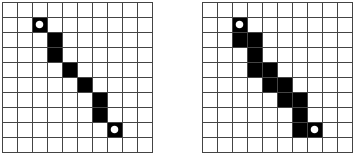
\includegraphics[width=6cm]{img/generated/line-grid.pdf}
\vskip 1.5ex

Finally, if we have code that draws a line between two arbitrary points, we might as well use it to also define a \lstinline`line` tool, which draws a straight line between the start and end of a drag.
